\documentclass[10pt]{article}

\usepackage[utf8]{inputenc}

\usepackage{tabularx}
\usepackage{amsmath}
\usepackage{amssymb}
\usepackage{geometry}
\geometry{a4paper, top=25mm, left=30mm, right=25mm, bottom=30mm,
         headsep=10mm, footskip=12mm}

\usepackage{graphicx}
\usepackage{url}
\usepackage[pdftex,colorlinks=true,citecolor=blue,urlcolor=blue,linkcolor=blue]{hyperref}
\usepackage{color}
\usepackage{xcolor}
\usepackage{tabularx}
\usepackage{listings}
\usepackage{parcolumns}
\usepackage{longtable}
\usepackage[margin=10pt]{caption}

% set the title
\title{\begin{tabular}{p{11cm}}\centering
Machine Learning with OpenCV2
\end{tabular}}

% contact details
\author{Philipp Wagner\\\href{http://www.bytefish.de}{http://www.bytefish.de}}

% colors for syntax highlightning
\definecolor{darkblue}{rgb}{0,0,.6}
\definecolor{darkred}{rgb}{.6,0,0}
\definecolor{darkgreen}{rgb}{0,.6,0}
\definecolor{red}{rgb}{.98,0,0}


% Listings Style
\lstset{
	numberstyle=\footnotesize, 
	basicstyle=\footnotesize\ttfamily
	numbers=left, 
	numbersep=5pt, 
	frame=single
}

% Add basic syntax highlightning to C++
\lstset{
	numberstyle=\footnotesize, 
	basicstyle=\footnotesize\ttfamily,
	numbers=none, 
	numbersep=5pt, 
	frame=single,
	breaklines=true,
	showspaces=false,
	showstringspaces=false,
	showtabs=false,
	tabsize=2,
}

\lstloadlanguages{C++}
\lstset{
	language=C++,
  commentstyle=\footnotesize\ttfamily\color{darkgreen},
  keywordstyle=\footnotesize\ttfamily\color{darkblue},
  stringstyle=\footnotesize\ttfamily\color{darkred},
}

\lstdefinelanguage{cmake}{
	morekeywords={cmake_minimum_required, project, find\_package, add\_executable, target\_link\_libraries},
	sensitive=false,
	morecomment=[l]{\#},
}

% change vertical space of itemize, description and enumeration environments
\let\olditemize=\itemize
   \def\itemize{\olditemize\setlength{\itemsep}{-0.5ex}}
\let\oldenumerate=\enumerate
   \def\enumerate{\oldenumerate\setlength{\itemsep}{-0.5ex}}
\let\olddescription=\description
   \def\description{\olddescription\setlength{\itemsep}{-0.5ex}}
   
% don't indent sections
\setlength{\parindent}{0pt}

\begin{document}

\maketitle
\tableofcontents

% include sections
\section{Introduction}

This document covers the Machine Learning API of the OpenCV2 C++ API. It helps you with setting up your system, gives a brief introduction into Support Vector Machines and Neural Networks and shows how it's implemented with OpenCV. Machine Learning is a branch of Artificial Intelligence and concerned with the question how to make machines able to learn from data. The core idea is to enable a machine to make intelligent decisions and predictions, based on experiences from the past. Algorithms of Machine Learning require interdisciplinary knowledge and often intersect with topics of statistics, mathematics, physics, pattern recognition and more.

\href{http://opencv.willowgarage.com}{OpenCV2} comes with a machine learning library for:
\begin{itemize}
 \item Decision Trees
 \item Boosting
 \item Support Vector Machines
 \item Expectation Maximization
 \item Neural Networks
\end{itemize}

\href{http://opencv.willowgarage.com}{OpenCV (Open Source Computer Vision)} is a popular computer vision library started by \href{http://www.intel.com}{Intel} in 1999. The cross-platform library sets its focus on real-time image processing and includes patent-free implementations of the latest computer vision algorithms. In 2008 \href{http://www.willowgarage.com}{Willow Garage} took over support and OpenCV 2.3.1 now comes with a programming interface to C, C++, \href{http://www.python.org}{Python} and \href{http://www.android.com}{Android}. OpenCV is released under a BSD license, so it is used in academic and commercial projects such as \href{http://www.google.com/streetview}{Google Streetview}.

Please don't copy and paste the code from this document, the project has been uploaded to \url{http://www.github.com/bytefish/opencv}. All code is released under a \href{http://www.opensource.org/licenses/bsd-license}{BSD license}, so feel free to use it for your projects.

\section{Installation Guide}

This installation guide explains how to install the software for this document. \href{http://www.cmake.org}{CMake} is used as build system for the examples, \href{http://www.mingw.org}{MinGW (Minimalist GNU for Windows)} is used as the compiler for Windows and OpenCV2 is compiled from source. There are binaries for OpenCV2 already, so why is it useful to build it from source at all? Your architecture may not be supported by the binaries, your toolchain may differ or the OpenCV version in your repository may not be the latest. Please note: You can always use the binaries supplied by WillowGarage or the binaries supplied by your distribution if they work for you.

The following guide was tested on Microsoft Windows XP SP3 and Ubuntu 10.10.

\subsection{Installing CMake}
\label{ssection:cmake}

\lstset{
	language=sh,
}

\href{http://www.cmake.org}{CMake} is an open-source, cross-platform build system. It manages the build process in a compiler-independent manner and is able to generate native build environments to compile the source code (\href{http://www.gnu.org/software/make/manual/}{Make}, \href{http://developer.apple.com/technologies/tools/}{Apple Xcode}, \href{http://www.microsoft.com/visualstudio/en-us}{Microsoft Visual Studio}, \href{http://www.mingw.org}{MinGW}, $\ldots$). Projects like \href{http://opencv.willowgarage.com}{OpenCV}, \href{http://www.kde.org}{KDE} or \href{http://www.blender.org}{Blender 3D} recently switched to CMake due to its flexibility. The CMake build process itself is controlled by configuration files, placed in the source directory (called \lstinline|CMakeLists.txt|). Each \lstinline|CMakeLists.txt| consists of CMake commands in the form of \lstinline|COMMAND(arguments...)|, that describe how to include header files, build libraries and executables. Please see the \href{http://www.cmake.org/cmake/help/cmake-2-8-docs.html}{CMake Documentation} for a list of available commands.

A Windows installer is available at \href{http://www.cmake.org/cmake/resources/software.html}{cmake.org/resources/software.html} (called \lstinline|cmake-<version>-win32-x86.exe|). Make sure to select \textit{"Add CMake to the system PATH for all users"} during setup or manually add it, so you can use \lstinline|cmake|, \lstinline|ccmake| and the \lstinline|cmake-gui| from command line (see \href{http://support.microsoft.com/kb/310519}{Microsoft Support: How To Manage Environment Variables in Windows XP} for details). Linux users should check the repository of their distribution, because the CMake binaries are often available already. 

If CMake is not available one can build it from source by:

\begin{lstlisting}
./bootstrap
make 
make install
\end{lstlisting}

Or install generic Linux binaries (called \lstinline|cmake-<version>-<os>-<architecture>.sh|):

\begin{lstlisting}
sudo sh cmake-<version>-<os>-<architecture>.sh --prefix=/usr/local 
\end{lstlisting}

\subsection{Installing MinGW}
\label{ssection:mingw}

\href{http://www.mingw.org}{MinGW (Minimalist GNU for Windows)} is a port of the \href{http://gcc.gnu.org}{GNU Compiler Collection (GCC)} and can be used for the development of native \href{http://www.microsoft.com/windows}{Microsoft Windows} applications. The easiest way to install MinGW is to use the automated mingw-get-installer \href{http://sourceforge.net/projects/mingw/files/Automated\%20MinGW\%20Installer/mingw-get-inst/}{from sourceforge.net/projects/mingw/files/Automated MinGW Installer/mingw-get-inst/} (called \textit{mingw-get-inst-20101030.exe} at time of writing this). If the path to the download changes, please navigate there from \href{http://www.mingw.org}{mingw.org}.

Make sure to select \textit{"C++ Compiler"} in the \textit{Compiler Suite} dialog during setup. Since MinGW doesn't add its binaries to the Windows PATH environment, you'll need to manually add it. The MinGW Page says: \textit{Add }\lstinline|C:\MinGW\bin|\textit{ to the PATH environment variable by opening the System control panel, going to the Advanced tab, and clicking the Environment Variables button. If you currently have a Command Prompt window open, it will not recognize the change to the environment variables; you will need to open a new Command Prompt window to get the new PATH.}

Linux users should install \href{http://gcc.gnu.org/}{gcc} and \href{http://www.gnu.org/software/make/}{make} (or a build tool supported by CMake) from the repository of their distribution. In Ubuntu the \lstinline|build-essential| package contains all necessary tools to get started, in Fedora and SUSE you'll need to install it from the available development tools.

\subsection{Building OpenCV}

Please skip this section if you are using the OpenCV binaries supplied by WillowGarage or your distribution. To build OpenCV you'll need CMake (see section \ref{ssection:cmake}), a C/C++ compiler (see section \ref{ssection:mingw}) and the OpenCV source code. At time of writing this, the latest OpenCV sources are available at \url{http://sourceforge.net/projects/opencvlibrary/}. I've heard the OpenCV page will see some changes soon, so if the sourceforge isn't used for future versions anymore navigate from the official page: \url{http://opencv.willowgarage.com}.

In this guide I'll use \href{http://sourceforge.net/projects/opencvlibrary/files/opencv-win}{OpenCV 2.3.0} for Windows and \href{http://sourceforge.net/projects/opencvlibrary/files/opencv-unix}{OpenCV 2.3.1} for Linux. If you need the latest Windows version download the \href{http://sourceforge.net/projects/opencvlibrary/files/opencv-win/}{superpack}, which includes binaries and sources for Windows.

\subsubsection*{Create the build folder}

First of all extract the source code to a folder of your choice, then open a terminal and \lstinline|cd| into this folder. Then create a folder \lstinline|build|, where we will build OpenCV in:

\begin{lstlisting}
mkdir build
cd build
\end{lstlisting}

\subsubsection*{Build OpenCV in Windows}

Now we'll create the Makefiles to build OpenCV. You need to specify the path you want to install OpenCV to (e.g. \lstinline|C:/opencv|), preferrably it's not the source folder. Note, that CMake expects a slash (\lstinline|/|) as path separator. So if you are using Windows you'll now write:

\begin{lstlisting}
cmake -G "MinGW Makefiles" -D:CMAKE_BUILD_TYPE=RELEASE -D:BUILD_EXAMPLES=1 -D:CMAKE_INSTALL_PREFIX=C:/opencv ..
mingw32-make 
mingw32-make install
\end{lstlisting}

Usually CMake is good at guessing the parameters, but there are a lot more options you can set (for Qt, Python, ..., see \href{http://opencv.willowgarage.com/wiki/InstallGuide}{WillowGarage's Install Guide} for details). It's a good idea to use the \lstinline|cmake-gui| to see and set the available switches. For now you can stick to the Listing, it works fine for Windows and Linux.

Better get a coffee, because OpenCV takes a while to compile! Once it is finished and you've decided to build dynamic libraries (assumed in this installation guide), you have to add the \lstinline|bin| path of the installation to Windows \lstinline|PATH| variable (e.g. \lstinline|C:/opencv/bin|). If you don't know how to do that, see \href{http://support.microsoft.com/kb/310519}{Microsoft Support: How To Manage Environment Variables in Windows XP} for details.

\subsubsection*{Build OpenCV in Linux}
Creating the Makefiles in Linux is (almost) similar to Windows. Again choose a path you want to install OpenCV to (e.g. \lstinline|/usr/local|), preferrably it's not the source folder.

\begin{lstlisting}[numberstyle=\footnotesize, numbers=left]
cmake -D CMAKE_BUILD_TYPE=RELEASE -D BUILD_EXAMPLES=1 -D CMAKE_INSTALL_PREFIX=/usr/local ..
make 
sudo make install
\end{lstlisting}

\subsubsection*{Sample CMakeLists.txt}
Once CMake is installed a simple \lstinline|CMakeLists.txt| is sufficient for building an OpenCV project (this is the build file for the example in this document):

\lstset{
	language=cmake,
}
\begin{lstlisting}
CMAKE_MINIMUM_REQUIRED( VERSION 2.8 )
PROJECT( ml_opencv )
FIND_PACKAGE( OpenCV REQUIRED )
ADD_EXECUTABLE( ml main.cpp )
TARGET_LINK_LIBRARIES(ml ${OpenCV_LIBS})
\end{lstlisting}

To build and run the project one would simply do (assuming we're in the folder with \lstinline|CMakeLists.txt|):

\lstset{
	language=sh,
}
\begin{lstlisting}
# create build directory 
mkdir build
# ... and cd into
cd build
# generate platform-dependent makefiles
cmake ..
# build the project
make
# run the executable
./ml
\end{lstlisting}

Or if you are on Windows with MinGW you would do:

\begin{lstlisting}
mkdir build
cd build
cmake -G "MinGW Makefiles" ..
mingw32-make
ml.exe
\end{lstlisting}

\section{Random Numbers in OpenCV}
Each thread in OpenCV has access to a default random number generator \lstinline|cv::theRNG()|. For a single pass the seed for the random number generator doesn't have to be set, but if many random numbers have to be generated (for example in a loop) the seed has to be set.

This can be done by assigning the local time to the random number generator:

\begin{lstlisting}
 cv::theRNG() = cv::RNG(time(0))
\end{lstlisting}

\subsection{Uniform Distribution}
Uniform Distributions can be generated in OpenCV with the help of \textit{cv::randu}. The signature of \textit{cv::randu} is:
\begin{lstlisting}[language=C++]
void randu(Mat& mtx, const Scalar& low, const Scalar& high);
\end{lstlisting}
Where
\begin{itemize}
 \item \textbf{mtx} is the Matrix to be filled with uniform distributed random numbers
 \item \textbf{low} is the inclusive lower boundary of generated random numbers
 \item \textbf{high} is the exclusive upper boundary of generated random numbers
\end{itemize}


\subsection{Normal Distribution}
Normal Distribution can be generated in OpenCv with the help of \textit{cv::randn}.
\begin{lstlisting}[language=C++]
void randn(Mat& mtx, const Scalar& mean, const Scalar& stddev);
\end{lstlisting}
Where
\begin{itemize}
 \item \textbf{mtx} is the Matrix to be filled with normal distributed random numbers
 \item \textbf{mean} the mean value of the generated random numbers
 \item \textbf{stddev} the standard deviation of the generated random numbers
\end{itemize}

\subsection{Bivariate Gaussian Distribution}

Multivariate normal distributions can be generated with the C API by using \textit{cvRandMVNormal} from the Machine Learning library. However this function seems to have no C++ equivalent yet, so in order to generate random numbers for the bivariate case one can also use the function given in \ref{lst:bivar}.

\begin{lstlisting}[language=C++, caption=bivariate\_gaussian dstribution, label=lst:bivar]
void bivariate_gaussian(float mu_x, float sigma_x, float mu_y, float sigma_y, float rho, cv::Mat &x, cv::Mat &y) {
  assert(x.rows == y.rows && x.rows > 0);

  int n = x.rows;

  randn(x, mu_x, sigma_x);

  cv::Mat r(n,1, CV_32FC1);
  cv::theRNG() = cv::RNG(time(0));

  randn(r, 0, 1);
  for(int i = 0; i < n; i++) {
    y.at<float>(i, 0) = sqrt(sigma_y*sigma_y - (rho * sigma_y)*(rho * sigma_y)) * r.at<float>(i, 0) + mu_y;
    y.at<float>(i, 0) = y.at<float>(i,0) + rho * sigma_y/sigma_x * (x.at<float>(i,0) - mu_x);
}
\end{lstlisting}


\section{Preparing the Training and Test Dataset for OpenCV ML}
In the C++ Machine Learning API of OpenCV training and test data is given as a \lstinline|cv::Mat| matrix. The constructor of \lstinline|cv::Mat| is defined as:
\begin{lstlisting}[language=C++]
Mat::Mat(int rows, int cols, int type);
\end{lstlisting}
Where
\begin{itemize}
 \item rows is the number of samples (for all classes!)
 \item columns is the number of dimensions
 \item type is the image type
\end{itemize}

In the machine learning library of OpenCV each row or column in the training data is a n-dimensional sample. The default ordering is row sampling and class labels are given in a matrix with equal length (one column only, of course). 

\begin{lstlisting}[language=C++]
cv::Mat trainingData(numTrainingPoints, 2, CV_32FC1);
cv::Mat testData(numTestPoints, 2, CV_32FC1);

cv::randu(trainingData,0,1);
cv::randu(testData,0,1);

cv::Mat trainingClasses = labelData(trainingData, equation);
cv::Mat testClasses = labelData(testData, equation);
\end{lstlisting}

Since only binary classification problems are considered the function \lstinline|f| returns the classes $-1$ and $1$ for a given two-dimensional data point:

\begin{lstlisting}[language=C++]
// function to learn
int f(float x, float y, int equation) {
  switch(equation) {
  case 0:
    return y > sin(x*10) ? -1 : 1;
    break;
  case 1:
    return y > cos(x * 10) ? -1 : 1;
    break;
  case 2:
    return y > 2*x ? -1 : 1;
    break;
  case 3:
    return y > tan(x*10) ? -1 : 1;
    break;
  default:
    return y > cos(x*10) ? -1 : 1;
  }
}
\end{lstlisting}

And to label data one can use the function \lstinline|labelData|:
\begin{lstlisting}
cv::Mat labelData(cv::Mat points, int equation) {
  cv::Mat labels(points.rows, 1, CV_32FC1);
  for(int i = 0; i < points.rows; i++) {
    float x = points.at<float>(i,0);
    float y = points.at<float>(i,1);
    labels.at<float>(i, 0) = f(x, y, equation);
  }
  return labels;
}
\end{lstlisting}
\section{Support Vector Machines (SVM)}
Support Vector Machines were first introduced by Vapnik and Chervonenkis in \cite{VC74}. The core idea is to find the optimal hyperplane to seperate a dataset, while there are theoretically infinite hyperplanes to seperate the dataset. A hyperplane is chosen, so that the distance to the nearest datapoint of both classes is maximized (Figure \ref{fig:maximum_margin}). The points spanning the hyperplane are the \textit{Support Vectors}, hence the name \textit{Support Vector Machines}. \cite{VC95}

\begin{figure}
\begin{center}
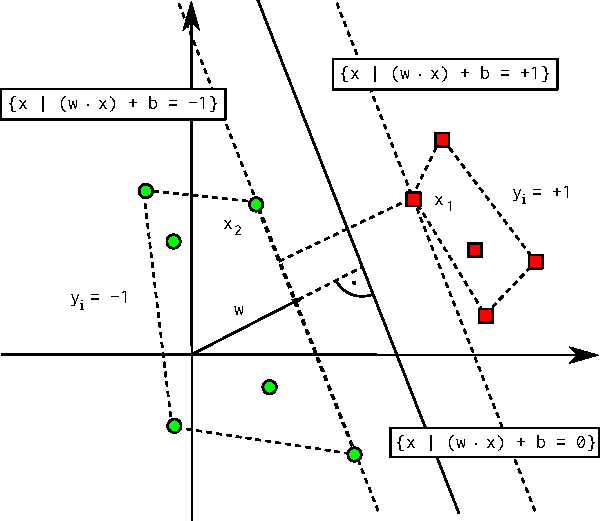
\includegraphics[scale=0.7]{img/svm/margin.pdf}
 % margin.pdf: 289x250 pixel, 72dpi, 10.20x8.82 cm, bb=0 0 289 250
\end{center}
 \caption{Maxmimum Margin Classifier.}
 \label{fig:maximum_margin}
\end{figure}

\subsection{Definition}
Given a Set of Datapoints $\mathcal{D}$:

$$\mathcal{D} = \left\{(x_i, y_i) | x_i \in \mathbb{R}^p, y_i \in \left\{-1,1\right\}\right\}_{i=1}^n$$
where
\begin{itemize}
 \item $x_i$ is a point in p-dimensional vector
 \item $y_i$ is the corresponding class label
\end{itemize}
We search for $\omega \in \mathbb{R}^n$ and bias $b$, forming the Hyperplane H:
$$\omega^T x + b = 0$$
that seperates both classes so that:
$$ \omega^T x + b = 1,\mbox{if } y = 1 $$
$$ \omega^T x + b = -1, \mbox{if } y = -1 $$

The optimization problem that needs to be solved is:
$$\mbox{min } \frac{1}{2}\omega^T \omega$$
subject to:
$$\omega^T x + b \geq 1, y = 1$$
$$\omega^T x + b \leq 1, y = -1 $$

Such quadratic optimization problems can be solved with standard solvers, such as \htmladdnormallink{GNU Octave}{www.gnu.org/software/octave} or \htmladdnormallink{Matlab}{www.mathworks.com/products/matlab}.

\subsubsection{Non-linear SVM}
The kernel trick is used for classifying non-linear datasets. It works by transforming data points into a higher dimensional feature space with a \textit{kernel function}, where the dataset can be seperated again (see Figure \ref{fig:kernel_trick}).


\begin{figure}[ht!]
\begin{center}
 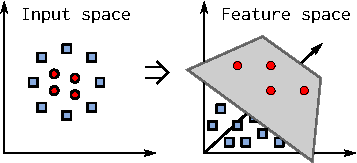
\includegraphics[scale=1.3]{img/svm/input_space2.pdf}
 \caption{Kernel Trick}
 \label{fig:kernel_trick}
 % input_space2.pdf: 1179666x1179666 pixel, 0dpi, infxinf cm, bb=
\end{center}
\end{figure}


Commonly used kernel functions are \textit{RBF kernels}:
$$k(x,x') = exp(\frac{\|x-x'\|^2}{\sigma^2})$$ 
or \textit{polynomial kernels}:
$$k(x,x') = (x \cdot x')^d$$.



\subsection{SVM in OpenCV}
Parameters for a SVM have to be defined in the structure \textit{CvSVMParams}.

\subsubsection*{Parameters}
\begin{lstlisting}[language=C++, caption=Example CvSVMParams, label=lst:cvsvmparams]
CvSVMParams param = CvSVMParams();

param.svm_type = CvSVM::C_SVC;
param.kernel_type = CvSVM::LINEAR;

param.degree = 0; // for poly
param.gamma = 20; // for poly/rbf/sigmoid
param.coef0 = 0; // for poly/sigmoid

param.C = 7; // for CV_SVM_C_SVC, CV_SVM_EPS_SVR and CV_SVM_NU_SVR
param.nu = 0.0; // for CV_SVM_NU_SVC, CV_SVM_ONE_CLASS, and CV_SVM_NU_SVR
param.p = 0.0; // for CV_SVM_EPS_SVR

param.class_weights = NULL; // for CV_SVM_C_SVC
param.term_crit.type = CV_TERMCRIT_ITER | CV_TERMCRIT_EPS;
param.term_crit.max_iter = 1000;
param.term_crit.epsilon = 1e-6;
\end{lstlisting}
Where the parameters are (taken from the OpenCV documentation):
\begin{itemize}
 \item \lstinline|svm_type|
 \begin{itemize}
  \item \lstinline|CvSVM::C_SVC| n-class classification ($n \geq 2$), allows imperfect separation of classes with penalty multiplier C for outliers.
  \item \lstinline|CvSVM::NU_SVC| n-class classification with possible imperfect separation. Parameter nu (in the range $0\ldots1$, the larger the value, the smoother the decision boundary) is used instead of C.
  \item \lstinline|CvSVM::ONE_CLASS| one-class SVM. All the training data are from the same class, SVM builds a boundary that separates the class from the rest of the feature space.
  \item \lstinline|CvSVM::EPS_SVR| regression. The distance between feature vectors from the training set and the fitting hyper-plane must be less than p. For outliers the penalty multiplier C is used.
  \item \lstinline|CvSVM::NU_SVR| regression; nu is used instead of p. 
 \end{itemize}
\item \lstinline|kernel_type|
\begin{itemize}
 \item \lstinline|CvSVM::LINEAR| no mapping is done, linear discrimination (or regression) is done in the original feature space. It is the fastest option. $d(x,y) = x \cdot y == (x,y)$.
 \item \lstinline|CvSVM::POLY| polynomial kernel: $d(x,y) = (gamma * (x \cdot y) + coef0)^{degree}$.
 \item \lstinline|CvSVM::RBF| radial-basis-function kernel; a good choice in most cases: $d(x,y) = exp(-gamma*|x-y|^2)$.
 \item \lstinline|CvSVM::SIGMOID| sigmoid function is used as a kernel: $d(x,y) = tanh(gamma * (x \cdot y) + coef0)$.
\end{itemize}
 \item \lstinline|C, nu, p| Parameters in the generalized SVM optimization problem. 
\item \lstinline|class_weights| Optional weights, assigned to particular classes. They are multiplied by C and thus affect the misclassification penalty for different classes. The larger weight, the larger penalty on misclassification of data from the corresponding class.
\item \lstinline|term_criteria| Termination procedure for iterative SVM training procedure (which solves a partial case of constrained quadratic optimization problem)
 \begin{itemize}
  \item \lstinline|type| is either \lstinline|CV_TERMCRIT_ITER| or \lstinline|CV_TERMCRIT_ITER| 
  \item \lstinline|max_iter| is the maximum number of iterations in training.
  \item \lstinline|epsilon| is the error to stop training.
 \end{itemize}
\end{itemize}

\subsubsection*{Training}
Training can either be done by passing the vector with the training data and vector with the corresponding class labels to the constructor or the train method.
\begin{lstlisting}[language=C++]
CvSVM(const CvMat* _train_data, 
      const CvMat* _responses,
      const CvMat* _var_idx=0,
      const CvMat* _sample_idx=0,
      CvSVMParams _params=CvSVMParams());
\end{lstlisting}
where
\begin{itemize}
 \item \textbf{\_train\_data} is a Matrix with the n-dimensional feature vectors
 \item \textbf{\_responses} is a vector with the class for the corresponding feature vector
 \item \textbf{\_var\_idx} identifies features of interest (can be left empty for this example, in code: \texttt{cv::Mat()})
 \item \textbf{\_sample\_idx} identifies samples of interest (can be left empty for this example, in code: \texttt{cv::Mat()})
 \item \textbf{\_params} Parameter for the SVM from Listing \ref{lst:cvsvmparams}
\end{itemize}
This applies to the train method aswell:
\begin{lstlisting}[language=C++]
virtual bool train(const CvMat* _train_data, 
  const CvMat* _responses,
  const CvMat* _var_idx=0,
  const CvMat* _sample_idx=0,
  CvSVMParams _params=CvSVMParams() );
\end{lstlisting}

The \textit{train} methods of the SVM has some limitations (at time of writing this):

 \begin{itemize}
  \item Only \verb|CV_ROW_SAMPLE| is supported
  \item Missing measurements are not supported
 \end{itemize}
The \textit{train\_auto} method finds the best parameters with a Gridsearch and a k-fold cross validation. This method is available for OpenCV Versions $\geq$ 2.0.

\subsubsection*{Prediction}
Self explaining code.
\begin{lstlisting}[language=C++]
for(int i = 0; i < testData.rows; i++) {
	cv::Mat sample = testData.row(i);
	float result = svm.predict(sample);
}
\end{lstlisting}

\subsubsection*{Support Vectors}
The support vectors of a SVM can be obtained using the \lstinline|get_support_vector| function of the API:
\begin{lstlisting}[language=C++]
int svec_count = svm.get_support_vector_count();
for(int vecNum = 0; vecNum < svec_count; vecNum++) {
	const float* vec = svm.get_support_vector(vecNum);
}
\end{lstlisting}


A complete example for Support Vector Machines in OpenCV is given in the Appendix.

\section{Multi Layer Perceptron}
An Artificial Neural Network is a biological inspired computational model. \textit{Inputs} multiplied by \textit{weights} result in an \textit{activation} and form the \textit{output} of a network.

Research in Artificial Neural Networks (ANN) began in 1943, when McCulloch and Pitts gave a definition of a formal neuron in their paper \textit{"A Logical Calculus of the Ideas Immanent in Nervous Activity"} \cite{culloch1943}. In 1958 Rosenblatt invented the perceptron, which is a simple feedforward neural network. The downfall of the perceptron algorithm is that it only converges on lineary seperable datasets and is not able to solve non-lineary problems such as the XOR problem. This was proven by Minsky and Papert in their monograph \textit{"Perceptrons"}, but they showed that a two-layer feedforward architecture can overcome this limitation. It was until 1986 when Rumelhart, Hinton and Williams presented a learning rule for Aritificial Neural Networks with hidden units in their paper \textit{"Learning Internal Representations by Error Propagation"}. The original discovery of backpropagation is actually credited to Werbos who described the algorithm in his 1974 Ph.D. thesis at Havard University, see \cite{werbos1994} for the roots of backpropagation.

A detailed introduction to Pattern Recognition with Neural Networks is given by \cite{Bishop95}.

\subsection{Backpropagation}

\begin{enumerate}
 \item Initilaize weights with random values
 \item Present the input vector to the network
 \item Evaluate the output of the network after a forward propagation of the signal
 \item Calculate $\delta_j = (y_j - d_j)$ where $d_j$ is the target output of neuron $j$ and $y_j$ is the actual output $y_j = g(\sum_i{ w_{ij}x_i}) = (1 + e^{-\sum_i{w_{ij}x_i}})^{-1}$, (when the activation function is of a sigmoid type).
\item For all other neurons (from the first to the last layer) calculate $\delta_j = \sum_k{w_{jk} g'(x)\delta_k}$, where  $\delta_k$ is $\delta_j$ of the succeeding layer and $g'(x) = y_k(1-y_k)$
\item Update weights with $w_{ij}(t+1) = w_{ij}(t) - \eta y_i y_j(1-y_j) \delta_j$, where $\eta$ is the learning rate.
\item Termination Criteria. Goto Step 2 for a fixed number of iterations or an error.
\end{enumerate}

The network error is defined as:
$$E = \frac{1}{2} \sum_{j=1}^{m}{(d_j - y_j)^2} $$

\subsection{MLP in OpenCV}
A Multilayer Perceptron in OpenCV is an instance of \lstinline|CvANN_MLP|.

\begin{lstlisting}[language=C++]
CvANN_MLP mlp;
\end{lstlisting}

\subsubsection*{Parameters}
The performance of a Multilayer perceptron depends on its parameters. The parameters I use are given in Listing \ref{lst:nnparams}.

\begin{lstlisting}[label=lst:nnparams, language=C++]
CvTermCriteria criteria;
criteria.max_iter = 100;
criteria.epsilon = 0.00001f;
criteria.type = CV_TERMCRIT_ITER | CV_TERMCRIT_EPS;

CvANN_MLP_TrainParams params;
params.train_method = CvANN_MLP_TrainParams::BACKPROP;
params.bp_dw_scale = 0.05f;
params.bp_moment_scale = 0.05f;
params.term_crit = criteria;
\end{lstlisting}

Where the parameters are (taken from the OpenCV 1.0 documentation\footnote{\url{http://www.cognotics.com/opencv/docs/1.0/ref/opencvref_ml.htm}}):
\begin{itemize}

\item \lstinline|term_crit| The termination criteria for the training algorithm. It identifies how many iterations is done by the algorithm (for sequential backpropagation algorithm the number is multiplied by the size of the training set) and how much the weights could change between the iterations to make the algorithm continue. 

\item \lstinline|train_method| The training algoithm to use; can be one of \lstinline|CvANN_MLP_TrainParams::BACKPROP| (sequential backpropagation algorithm) or \lstinline|CvANN_MLP_TrainParams::RPROP| (RPROP algorithm, default value). 

\item \lstinline|bp_dw_scale|
    (Backpropagation only): The coefficient to multiply the computed weight gradient by. The recommended value is about 0.1.
\item \lstinline|bp_moment_scale|
    (Backpropagation only): The coefficient to multiply the difference between weights on the 2 previous iterations. This parameter provides some inertia to smooth the random fluctuations of the weights. It can vary from 0 (the feature is disabled) to 1 and beyond. The value 0.1 or so is good enough.
\item \lstinline|rp_dw0|
    (RPROP only): Initial magnitude of the weight delta. The default value is 0.1.
\item \lstinline|rp_dw_plus|
    (RPROP only): The increase factor for the weight delta. It must be >1, default value is 1.2 that should work well in most cases, according to the algorithm's author.
\item \lstinline|rp_dw_minus|
    (RPROP only): The decrease factor for the weight delta. It must be <1, default value is 0.5 that should work well in most cases, according to the algorithm's author.
\item \lstinline|rp_dw_min|
    (RPROP only): The minimum value of the weight delta. It must be >0, the default value is \lstinline|FLT_EPSILON|. 
\item \lstinline|rp_dw_max|
    (RPROP only): The maximum value of the weight delta. It must be >1, the default value is 50. 
\end{itemize}


\subsubsection*{Layers}
The purpose of a neural network is to generalize, which is the ability to approximate outputs for inputs not available in the training set. \cite{Sa02} While small networks may not be able to approximate a function, large networks tend to overfit and not find any relationship in data.\footnote{The model describes random error or noise instead of the relationship of the data.} It has been shown that, given enough data, a multi layer perceptron with one hidden layer can approximate any continuous function to any degree of accuracy.\cite{HSW92}

The number of neurons per layer is stored in a row-ordered \lstinline|cv::Mat|.

\begin{lstlisting}[language=C++]
cv::Mat layers = cv::Mat(4, 1, CV_32SC1);

layers.row(0) = cv::Scalar(2);
layers.row(1) = cv::Scalar(10);
layers.row(2) = cv::Scalar(15);
layers.row(3) = cv::Scalar(1);

mlp.create(layers);
\end{lstlisting}

\subsubsection*{Training}
The API for training a multilayer perceptron takes the training data, training classes and the structure for the parameters.

\begin{lstlisting}[language=C++]
mlp.train(trainingData, trainingClasses, cv::Mat(), cv::Mat(), params);
\end{lstlisting}

\subsubsection*{Prediction}
The API for the prediction is slightly different from the SVM API. Activations of the output layer are stored in a \lstinline|cv::Mat| response, simply because one can design neural networks with multiple neurons in the output layer.

Since the problem used in this example is a binary classification problem, it is sufficient to have only one neuron in the output layer. It is therefore the only activation to check.

\begin{lstlisting}[language=C++]
mlp.predict(sample, response);
float result = response.at<float>(0,0);
\end{lstlisting}
\section{Evaluation}
In this section the following algorithms will be used for classification:
\begin{itemize}
 \item Support Vector Machine
 \item Multi Layer Perceptron
 \item k-Nearest-Neighbor
 \item Normal Bayes
 \item Decision Tree
\end{itemize}

To evaluate a predictor it is possible to calculate its accuracy. For two classes it is given as:

$$Accuracy = \frac{\mbox{true positive}}{\mbox{true positive} + \mbox{false positive}}$$

The performance of Support Vector Machines and especially Neural Networks depend on the parameters chosen. In case of a neural network it is difficult to find the appropriate parameters and architecture. Designing an Artifical Neural Network is often more a rule of thumb and networks should be optimized iteratively starting with one hidden layer and few neurons. Parameters for a Support Vector Machine can be estimated using Cross Validation and Grid Search (both can be used as \lstinline|train_auto| in OpenCV $\geq$ 2.0).

In this evaluation parameters won't be optimized, remember to optimize the parameters yourself when using one of the algorithms.


\subsection{y = 2x}

\begin{tabular}{|c|c|}
\hline
Predictor &	 Accuracy\\ \hline\hline
Support Vector Machine &	0.99\\ \hline
Multi Layer Perceptron (2, 10, 15, 1) & 0.994\\ \hline
k-Nearest-Neighbor (k = 3) & 0.9825\\ \hline
Normal Bayes &	0.9425 \\ \hline
Decision Tree &	0.923\\ \hline
\end{tabular}

\subsubsection{Plot}
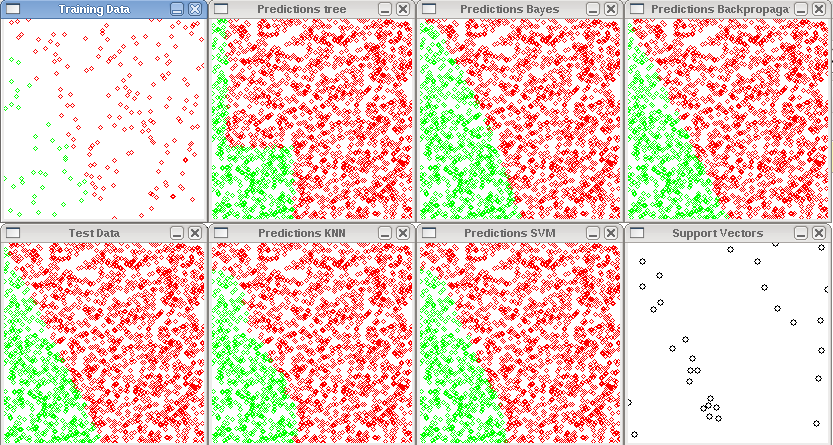
\includegraphics[scale=0.4]{img/eval/2x.png}

\subsection{y = sin(10x)}

\begin{tabular}{|c|c|}
\hline
Predictor &	Accuracy\\ \hline\hline
Support Vector Machine &	0.913\\ \hline
Multi Layer Perceptron (2, 10, 15, 1) & 0.6855\\ \hline
k-Nearest-Neighbor (k = 3) & 0.9\\ \hline
Normal Bayes & 0.632\\ \hline
Decision Tree &	0.886\\ \hline
\end{tabular}

\subsubsection{Plot}
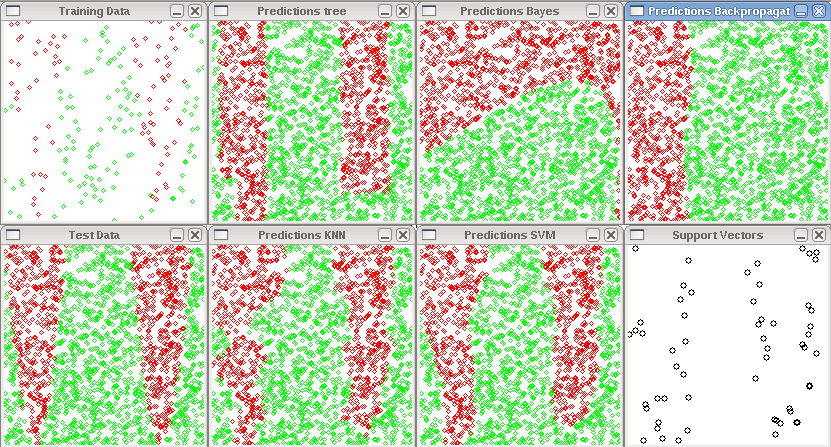
\includegraphics[scale=0.4]{img/eval/sin10x.png}

\subsection{y = tan(10x)}

\begin{tabular}{|c|c|}
\hline
Predictor &	Accuracy\\ \hline\hline
Support Vector Machine & 0.7815\\ \hline
Multi Layer Perceptron (2, 10, 15, 1) &	0.5115\\ \hline
k-Nearest-Neighbor (k = 3) & 0.8195\\ \hline
Normal Bayes &	0.542\\ \hline
Decision Tree &	0.9155\\ \hline
\end{tabular}

\subsubsection{Plot}
 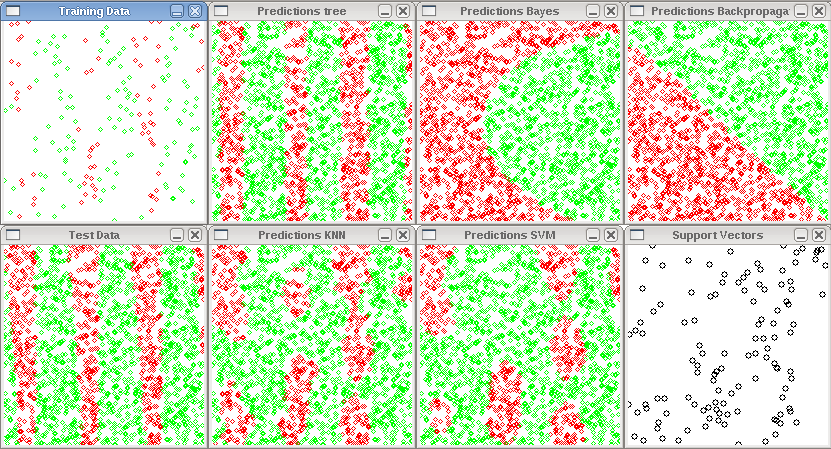
\includegraphics[scale=0.4]{img/eval/tan10x.png}


\appendix

\section{main.cpp}
\lstinputlisting[language=C++, caption=main.cpp]{../main.cpp}

% bibliography
\bibliography{bib/machinelearning}
\bibliographystyle{acm}

\end{document}
